\documentclass{article}
\usepackage[frenchb]{babel}
\usepackage[utf8]{inputenc}
\usepackage[T1]{fontenc}
\usepackage{graphicx}
\usepackage{float}


\title{Projet : Multicore Programming}
\author{Joachim Clayton, Master 1 ALMA}



\begin{document}

\renewcommand{\contentsname}{Sommaire} 


\maketitle
\date


\begin{figure}[h!]
   \centerline{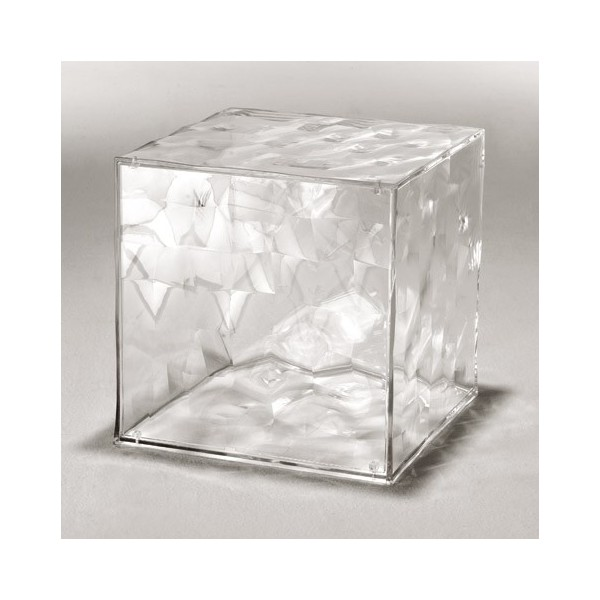
\includegraphics[width=400pt]{source/0.jpg}}
\end{figure}



\newpage

\tableofcontents

\newpage

\section{Introduction}

Ce projet a pour but de validé l'utilisation des technologies servant à la parallelisation d'un code séquentiel.

Le code séquentiel sur lequel nous travaillons à la base est un code permettant de trouver des solutions à ''Quel est l'interval contenant le minimum de cette fonction ?''
La ou les fonctions sont également représenté dans un espace en 3 dimension ( un cube) et l'algorithme fonctionne alors en divisant ce cube en 4 et en retressissant les zones de recherche afin de trouver le plus petit cube contenant le resultat (selon la précision que l'on aura donnée).

La division de ce cube et donc son traitement peut ainsi se réaliser de façon parallèle. 
\vspace{1cm}

\section{OpenMP}

Bien que cela soit demander dans la deuxième question et étant plus à l'aise avec openMP j'ai commencé par créer une version du code sequentiel en openmp.
Pour cela j'ai réalisé les modifications necessaires dans le makefile (modifiant aussi au passage pour la compilation du futur fichier mpi)

J'ai choisis d'utiliser le pragma omp parallel sections pour avoir une certaines sécurité au niveau du regroupement après l'exécution des differentes sections
Contrairement aux tasks qui me parraissait plus difficile à controler.

Comme le code séquentielle le stipule, le cube est coupé en 4 puis en 4 etc...
De ce faite, j'ai décidé d'alloué 4 thread chacun s'occupant d'un cube et c'est autour du traitement de chacun de ces 4 cube que l'on articule la parallèlisation.

Cependant il reste des affectations de variable précedement et il est important que ces parties restes bien en séquentielle, c'est pour cela que j'utilise le pragma omp critique.

Les performances du programme ''omp'' sont doublement plus rapide comparé à celle du ''seq''.


\section{MPI}

Au sujet d'MPI, j'ai réalisé la modification du make pour pouvoir réaliser la compilation du fichier MPI.
J'ai également réaliser l'initiation et le finalize du programme

Le but de ce programme est de faire en sorte de faire s'executer les parties du programme par plusieurs ordinateurs à la fois (plusieurs coeurs) en indiquant grâce à MPI qui fait quoi, quel ordinateur s'occupe de quoi.
Une fois chaque processus mis en marche avec la tâche qui leur ai confié, il faudra récupérer les informations et arriver à la solution rechercer grâce à un réduce.


\section{Conclusion}

Je n'ai pas réussi l'implémentation du MPI et beaucoup hésiter entre l'utilisation d'un MPI\_Bcast en indicant chaque machine puis un MPI\_Reduce ou par l'utilisation d'un processus qui gererai les resultats avec un if, else simple qui receverai les valeur si c'est le rang 0 et qui enverai les valeurs sinon par exemple.
Malheureusement étant sur windows pour la fin de ce projet, les tests ont été difficile.



\end{document}
